\documentclass[10pt]{article}
\usepackage{tikz}
\usetikzlibrary{shapes.geometric}

\begin{document}

\section{Cas 1}

\subsection{Situation de départ:}

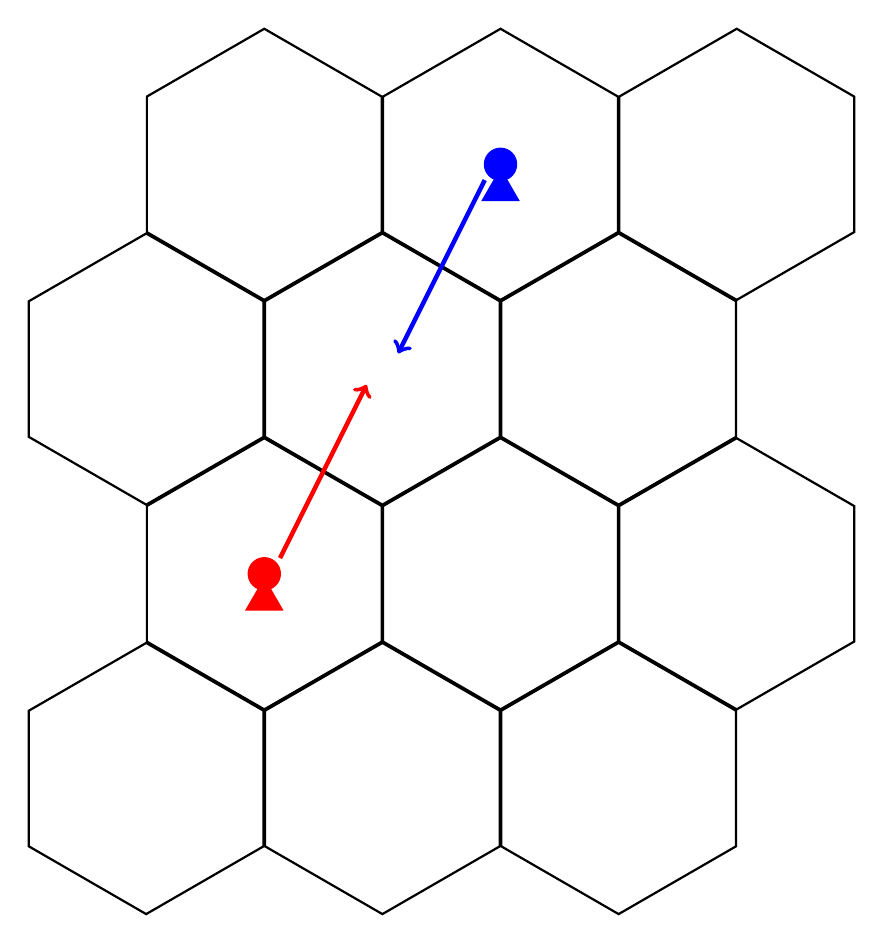
\begin{tikzpicture}[
monsterBody/.style={regular polygon, regular polygon sides=3, fill, very thick, inner sep=1mm, below},
monsterHead/.style={circle, fill, inner sep=1.5mm},
]

        \foreach \i in {0,..., 2}
                \foreach \j in {0, 2,..., 2} {
                        \path (3*\i, 2.6*\j) node[regular polygon, regular polygon sides=6, draw, thick, inner sep = 30, rotate = 90] (hexa) {};
			\path (3*\i-1.5, 2.6*\j-2.6) node[regular polygon, regular polygon sides=6, draw, thick, inner sep = 30, rotate = 90] (hexa) {};
                }

        \path (0, 0) node[monsterBody] (m1) [red] {};
        \path (0, 0) node[monsterHead] [red] {};
        \draw[->, red, ultra thick] (0.2, 0.2) -- (1.3, 2.4);
	\path (2*1.5, 2*2.6) node[monsterBody] [blue] {};
	\path (2*1.5, 2*2.6) node[monsterHead] [blue] {};
	\draw[->, blue, ultra thick] (2.8, 5) -- (1.7, 2.8);

\end{tikzpicture}

\newpage

\subsection{Egalite, rouge et bleu subisse un dégat:}%TODO degat pour les deux ou pas de degat?

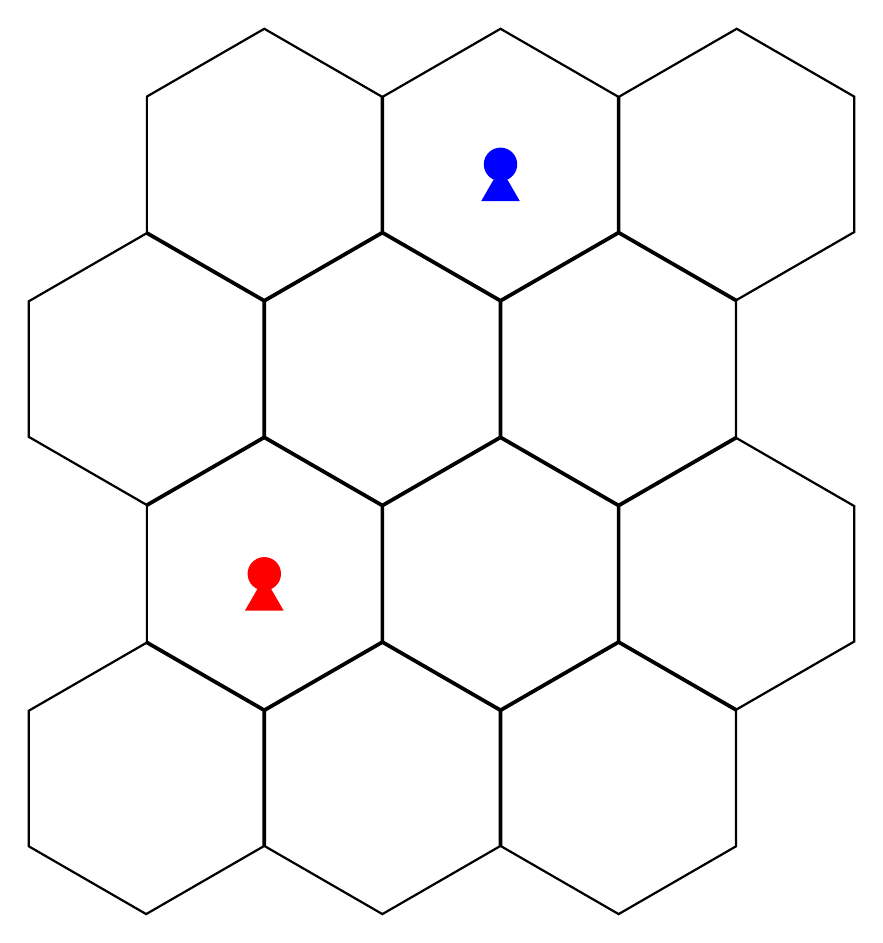
\begin{tikzpicture}[
monsterBody/.style={regular polygon, regular polygon sides=3, fill, very thick, inner sep=1mm, below},
monsterHead/.style={circle, fill, inner sep=1.5mm},
]

        \foreach \i in {0,..., 2}
                \foreach \j in {0, 2,..., 2} {
                        \path (3*\i, 2.6*\j) node[regular polygon, regular polygon sides=6, draw, thick, inner sep = 30, rotate = 90] (hexa) {};
			\path (3*\i-1.5, 2.6*\j-2.6) node[regular polygon, regular polygon sides=6, draw, thick, inner sep = 30, rotate = 90] (hexa) {};
                }

        \path (0, 0) node[monsterBody] (m1) [red] {};
        \path (0, 0) node[monsterHead] [red] {};
	\path (2*1.5, 2*2.6) node[monsterBody] [blue] {};
	\path (2*1.5, 2*2.6) node[monsterHead] [blue] {};

\end{tikzpicture}

\newpage

\subsection{Victoire de rouge, bleu subit un dégat}

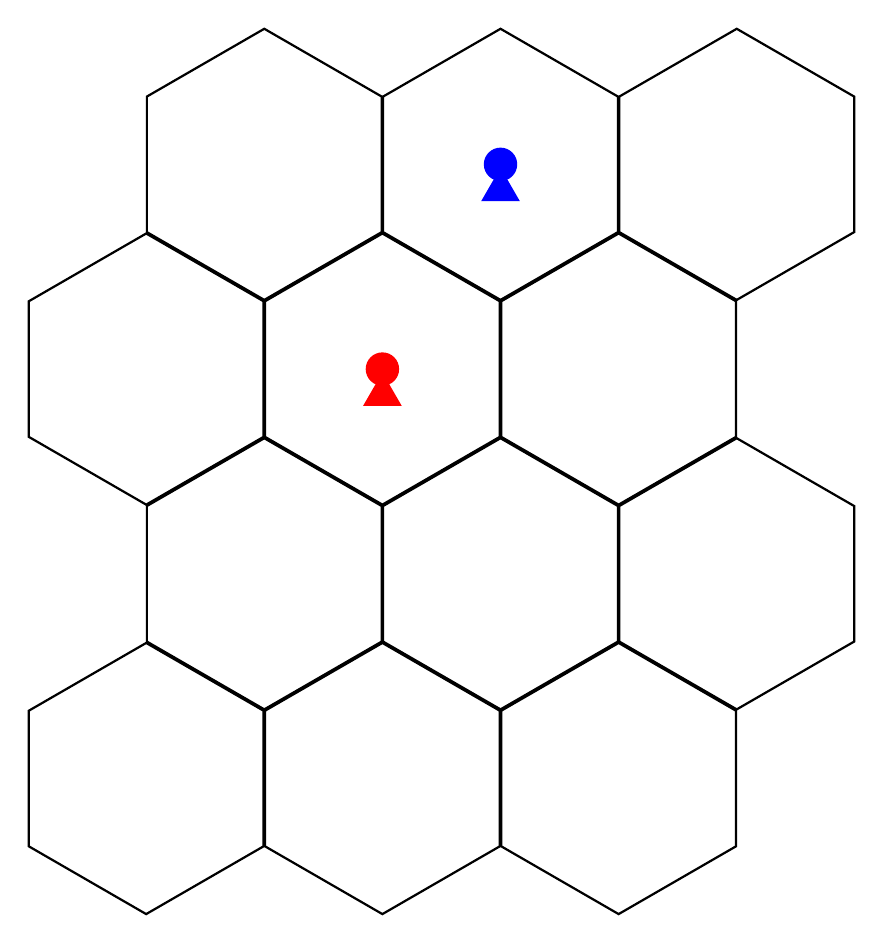
\begin{tikzpicture}[
monsterBody/.style={regular polygon, regular polygon sides=3, fill, very thick, inner sep=1mm, below},
monsterHead/.style={circle, fill, inner sep=1.5mm},
]

        \foreach \i in {0,..., 2}
                \foreach \j in {0, 2,..., 2} {
                        \path (3*\i, 2.6*\j) node[regular polygon, regular polygon sides=6, draw, thick, inner sep = 30, rotate = 90] (hexa) {};
			\path (3*\i-1.5, 2.6*\j-2.6) node[regular polygon, regular polygon sides=6, draw, thick, inner sep = 30, rotate = 90] (hexa) {};
                }

        \path (1.5, 2.6) node[monsterBody] (m1) [red] {};
        \path (1.5, 2.6) node[monsterHead] [red] {};
	\path (2*1.5, 2*2.6) node[monsterBody] [blue] {};
	\path (2*1.5, 2*2.6) node[monsterHead] [blue] {};

\end{tikzpicture}

\newpage

\begin{tikzpicture}[
monsterBody/.style={regular polygon, regular polygon sides=3, fill, very thick, inner sep=1mm, below},
monsterHead/.style={circle, fill, inner sep=1.5mm},
]

        \foreach \i in {0,..., 2}
                \foreach \j in {0, 2,..., 2} {
			\path (2*\i, 2*$\cos(\pi/6)$*\j) node[regular polygon, regular polygon sides=6, draw, thick, inner sep = 20, rotate = 90] {};
			\path (2*\i-1, 2*$\cos(\pi/6)$*\j-2*$\cos(\pi/6)$) node[regular polygon, regular polygon sides=6, draw, thick, inner sep = 20, rotate = 90] {};
                }

\end{tikzpicture}

\end{document}
